\begin{xmp}[Бифуркация Андронова-Копфа]
	\begin{flalign*}
		& \begin{cases}
			\dot x = \alpha x - y - x(x^2 + y^2) \\
			\dot y = x + \alpha y - y(x^2 + y^2) \\
		\end{cases} &\\
		& x = y = 0 \text{ равновесие. Откинем квадратичную часть.} &\\
		& \det(A - \lambda E) = \begin{vmatrix}
			\alpha - \lambda & - 1 \\
			1 & \alpha - \lambda \\
		\end{vmatrix} = \lambda^2 - 2\alpha\lambda + \alpha^2 + 1 &\\
		& \alpha < 0 \Rightarrow x = y = 0 \text{ --- устойчиво.} &\\
		& \alpha > 0 \Rightarrow x = y = 0 \text{ --- неустойчиво.} &\\
	\end{flalign*}
	\begin{figure}[H]
		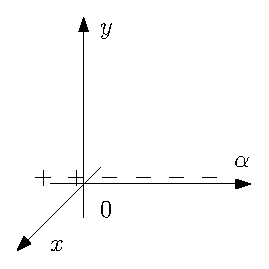
\includegraphics{5_1.eps}
	\end{figure}
	\begin{flalign*}
		& x = r\cos\varphi,\; y = r\sin\varphi &\\
		& \begin{cases}
			\dot r\cos\varphi - r\dot\varphi\sin\varphi = \alpha r \cos\varphi - r\sin\varphi - r\cos\varphi\cdot r^2 & | \cdot \cos\varphi\\
			\dot r\sin\varphi + r\dot\varphi\cos\varphi = r\cos\varphi + \alpha r\sin\varphi - r\sin\varphi\cdot r^2 & | \cdot \sin\varphi\\
		\end{cases} &\\
		& \begin{cases}
			\dot r = \alpha r - r^3  & (1)\\
			\dot \varphi = 1 \\
		\end{cases} &\\
		& r = 0,\; r = \pm\sqrt{\alpha} \text{ --- равносильные уравнению } (1). &\\
	\end{flalign*}
	\begin{figure}[H]
		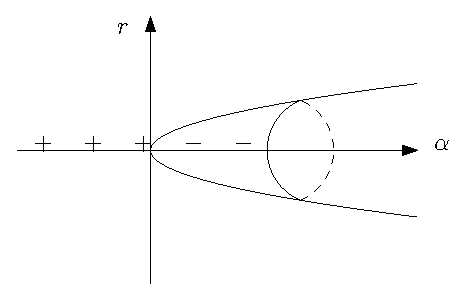
\includegraphics{5_2.eps}
	\end{figure}
	\begin{flalign*}
		& \delta r = r - \sqrt{\alpha} &\\
		& \delta \dot r = \dot r,\; r = \delta r + \sqrt{\alpha} &\\
		& (1) \Leftrightarrow \delta \dot r - (\delta r + \sqrt{\alpha})(-\delta r)(\delta r + 2\sqrt \alpha) = -2\alpha\delta r + O_2(\delta r) &\\
		& \delta r = o(r \pm \sqrt \alpha) \text{ --- устойчивое.}
	\end{flalign*}
	\begin{figure}[H]
		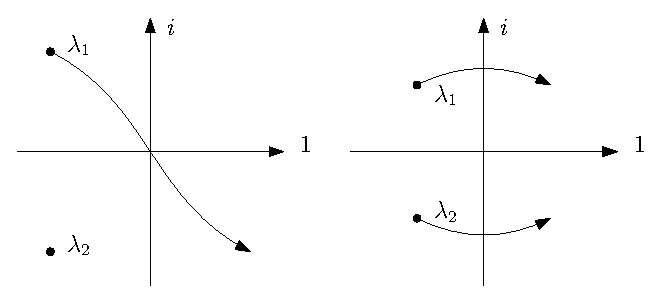
\includegraphics{5_3.eps}
		\caption*{1) Дивергенция. 2) Флаттер.}
	\end{figure}
\end{xmp}

\subsection{Малые Колебания}
\begin{flalign*}
& T = \frac{1}{2}(\Phi(\v q)\dv q, \dv q), \; \Pi(\v q), \; \v q = 0 \text{ --- положение равновесия} &\\
& \Pi(\v q) = \underbrace{\Pi(0)}_0 + \left( \left.\pd{\Pi}{\v q}\right|_{\v q = 0}, \v q \right) + \frac{1}{2}\left( \left.\pd{^2 \Pi}{\v q^2}\right|_{\v q = 0}, \v q \right) + O_3(\v q) &\\
& \left. \pd{^2 \Pi}{\v q^2} \right|_{\v q = 0} = c = const, \quad C = C^T &\\
& T = \frac{1}{2}\left(\left(\Phi(0) + O(\norm{\v q})\right)\dv q, \dv q\right) = \frac{1}{2}(A \dv q, \dv q) + O_3(\v q, \dv q) &\\
& A = \Phi(0) = const, \; A = A^T &\\
& L = \tilde L + O_3(\v q,\dv q),\; \tilde L = \frac{1}{2}(A\dv q, \dv q) - \frac{1}{2}(C\v q, \v q) &\\
& \pd{\tilde L}{\dv q} = \frac{1}{2}\underbrace{(A\dv q + A^T \dv q)}_{\text{Из 3 семестра}} = A \dv q, \quad \frac{\partial\tilde L}{\partial\v q} = -C\v q \text{ --- аналогично} &\\
& \frac{d}{dt}\pd{\tilde L}{\dv q} - \pd{\tilde L}{\v q} = 0 \Leftrightarrow \boxed{A\ddot{\v q} + C\v q = 0} &\\
& \text{$A$ положительно определена } \xrightarrow{\text{Из линейной алгебры}} \exists \v e_1, \ldots, \v e_n: \: A \rightarrow E, C \rightarrow k &\\
& \v q = \sum \xi_i \v e_i = u \v \xi, \tilde L = \frac{1}{2}(E \dv \xi, \dv \xi) - \frac{1}{2}(k \v \xi, \v \xi), &\\
& k = \diag(k_1, \ldots, k_n) &\\
& \text{Уравнения Лагранжа:} &\\
& \ddot{\v \xi} + k\v \xi = 0 \Rightarrow \begin{cases}
\ddot{\xi}_1 + k_1\xi_1 = 0 \\
\vdots \\
\ddot{\xi}_n + k_n\xi_n = 0 \\
\end{cases} &\\
& \text{Пусть } k_i = \omega_i^2 > 0 &\\
& k \text{ и } C \text{ --- положительно определены, } \v q = 0 (\v \xi = 0) \text{ --- устойчиво по теореме Лагранжа-Дирихле} &\\
& \ddot \xi_i + k_i \xi_i = 0 \quad \lambda^2 + k_i, \quad \lambda^2 + \omega_i^2 = 0 \quad \lambda = \pm \omega_i i &\\
& \xi_i = C_{1i} \sin \omega_i t + C_{2i}\cos \omega_i t = \alpha_i\sin(\omega_i t + \varphi_i) &\\
& \v q = \sum_{i = 1}^n \alpha_i \v e_i \sin(\omega_i t + \varphi_i)
\end{flalign*}

\begin{ass}
\begin{flalign*}
& \det (A \omega^2 - C) = 0 &\\
& \begin{cases}
A(\omega_i^2 - C) e_i = 0 \\
(A \v e_i, \v e_i) = 1 \\
\end{cases},
i = 1, \ldots, n
\end{flalign*}
\end{ass}
\begin{proof}
\begin{flalign*}
& 2\tilde \Pi = (C\v q, \v q) = (CU\v \xi, U\v \xi) = (U^TCU\v \xi, \v \xi) = (k\v \xi, \xi) \Leftrightarrow k = U^TCU &\\
& 2\tilde T = (A\dv q, \dv q) = (U^TAU\v \xi, \v \xi) = (E\dv \xi, \dv \xi) \Leftrightarrow &\\
& \Leftrightarrow E = U^TAU (\Leftrightarrow (A\v e_i, \v e_j) = \delta_{ij}) &\\
& k - k_iE = \diag(k_1 - k_i, \ldots, k_{i - 1} - k_i, 0, \ldots) &\\
& \det(k - k_iE) = 0 \Leftrightarrow \det(U^TCU - k_iU^TAU) = 0 \Leftrightarrow &\\
& \Leftrightarrow \det U^T \det(C - Ak_i)\det U = 0 \leftarrow\xrightarrow{\det U \neq 0} \det(Ak_i - C) = 0, \det(A \omega_i^2 - C) = 0 &\\
& 2) (k - k_iE)(0, \ldots, 0, \underbrace{1}_i, 0, \ldots)^T &\\
& (U^TC - k_iU^TA)\underbrace{U(0, \ldots, 0, 1, 0, \ldots, 0)^T}_{\v e_i} \qquad C\v q = \sum \v e_i\xi_i &\\
& U^T(C - \omega_i^2 A)\v e_i = 0 \Leftrightarrow (A\omega_i - C)\v e_i = 0 &\\
\end{flalign*}
\end{proof}

\begin{df}
$\det(A\omega^2 - C) = 0$ --- вековое уравнение (уравнение частот). $\omega_i$ --- частоты малых колебаний (собственные частоты).
\end{df}

\begin{cor}
Частоты малых колебаний не зависят от выбора обобщенных координат.
\end{cor}

\begin{df}
Если $(A\omega_i^2 - C)\v U_i = 0$, то $\v U_i$ --- амплитудный вектор, соответствующий частоте $\omega_i$.
\end{df}

\begin{ntc}
$\v U_i = \beta_i \v e_i,\; \beta_i = const$
\end{ntc}

\begin{flalign*}
& \v q = \sum_{i = 1}^n \tilde \alpha_i \v U_i \sin(\omega_i t + \varphi_i) &\\
\end{flalign*}

\begin{cor}
\begin{enumerate}
\item Ортогональность
\[
	(A\v U_i, \v U_j) = 0, \; i \neq j
\]
\item Линейная независимость
\begin{gather*}
C_1U_1 + \ldots + C_nU_n = 0 \\
0 + \ldots + (A\v U_i, C_i \v U_i) + \ldots + 0 = 0 \Leftrightarrow C: (A\v U_i, \v U_i) = 0 \Leftrightarrow C_i = 0 \\
(A\v U, \v U) = 0 \Leftrightarrow \v U = 0
\end{gather*}
\end{enumerate}
\end{cor}

\begin{ntc}
$\tilde \alpha, \varphi$ --- определяются начальными условиями.
\end{ntc}

\begin{flalign*}
I.\;\; &\tilde \alpha_i = 0, \quad \forall i \neq m: \v q = \tilde \alpha_m \v U_m \sin(\omega_m t + \varphi_m) &\\
& \text{главные (нормальные) колебания} &\\
Ia.\;& \text{Кратные частоты } \omega_1 = \omega_2 = \omega &\\
& k = \diag(\omega_1^2, \omega_2^2, \ldots) &\\
& \begin{cases}
\ddot \xi_1 + \omega^2 \xi_1 = 0 \\
\ddot \xi_2 + \omega^2 \xi_2 = 0
\end{cases} &\\
& (A\omega^2 - C)\v U = 0 &\\
& U = C_1\v U_1 + C_2\v U_2 &\\
II.\;& \exists k_m = 0 &\\
& \ddot \xi_m = 0,\; \xi_m = C_1t + C_2 &\\
III.& \exists k_m < 0, \v q = 0 (\xi = 0) \text{ --- неустойчиво.} &\\
& \ddot \xi_m + k_m\xi_m = 0 &\\
& \lambda^2 = -k_m > 0 &\\
& \lambda = \pm \sqrt{-k_m}
\end{flalign*}

\begin{teo}
Если $\Pi^{(2)}_{(0)}$ не имеет даже нестрогий минимум, то $\v q = 0$ неустойчиво.
\end{teo}
\begin{proof}
\begin{flalign*}
& \underline{n = 1} \text{ уже доказано} &\\
& \underline{n > 1} \quad \v q \rightarrow \v \xi &\\
& \begin{cases}
\ddot \xi_1 + k_1\xi_1 = 0 \\
\vdots \\
\ddot \xi_n + k_n\xi_n = 0 \\
\end{cases} &\\
& \exists k_m < 0: \ddot \xi_m + k_m \xi_m = 0 \text{ ---||--- } &\\
\end{flalign*}
\end{proof}

\subsection{Вынужденные колебания в линейных системах}
\begin{flalign*}
& \ddot x + \omega_0^2x = f\cos\omega t &\\
& x = x_{\text{одн}} + x_\text{ч} &\\
& x_{\text{одн}} = C_1 \sin \omega_0 t + C_2\cos \omega_0t &\\
& 1)\; \omega \neq \omega_0: x_\text{ч} = \alpha\sin \omega t + \beta\cos \omega t \quad /\; \omega_0^2 &\\
& \qquad \dot x_\text{ч} = \alpha\omega\cos\omega t - \beta\omega\sin\omega t \quad /\; 0 &\\
& \qquad \ddot x_\text{ч} = -\alpha\omega^2\sin\omega t - \beta\omega^2\cos\omega t \quad /\; 1 &\\
& \begin{cases}
\alpha \omega_0^2 - \alpha \omega^2 = 0 \\
\beta \omega_0^2 - \beta \omega^2 = f \\
\end{cases}
\Rightarrow
\begin{cases}
\alpha = 0 \\
\beta = \frac{f}{\omega_0^2 - \omega^2}
\end{cases} &\\
& x = C_1\sin \omega_0t + C_2\cos \omega_0 t + \frac{f}{\omega_0^2 - \omega^2}\cos\omega t
\end{flalign*}
\begin{figure}[H]
	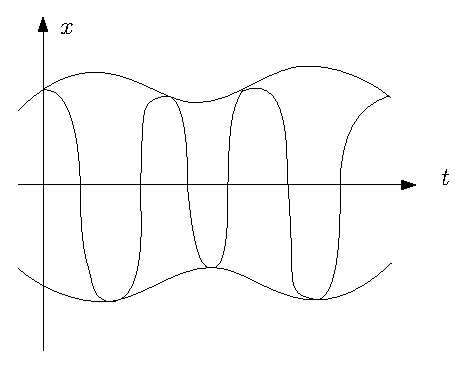
\includegraphics{5_4.eps}
	\caption*{Биения.}
\end{figure}
\begin{flalign*}
& 2)\; \omega = \omega_0 \quad x_\text{ч} = \alpha t \sin \omega_0 t &\\
& \qquad \dot x_\text{ч} = \alpha \sin\omega_0t + \alpha \omega_0t\cos \omega_0t &\\
& \qquad \ddot x_\text{ч} = \alpha \omega_0 \cos \omega_0 t - \alpha \omega_0 t \sin \omega_0 t \Rightarrow 2\alpha \omega_0 = f \Rightarrow \alpha = \frac{f}{2\omega_0} &\\
& x = C_1 \sin \omega_0t + C_2\cos \omega_0t + \frac{f}{2\omega_0}t \sin \omega_0t
\end{flalign*}
\begin{figure}[H]
	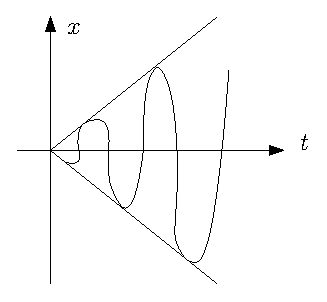
\includegraphics{5_5.eps}
	\caption*{Резонанс.}
\end{figure}
\begin{flalign*}
& A\ddot{\v q} + C \v q = \v Q, \quad \v Q = \v F \cos \omega t &\\
& \v q = U \v \xi, \quad A \rightarrow E, \; C \rightarrow K &\\
& (\v Q, \delta \v q) = (\v Q, U\delta \v \xi) = (U^T\v Q, \delta \v \xi) = (\v Q \delta \v \xi) &\\
& \tilde Q = U^T \tilde Q &\\
\end{flalign*}